\documentclass{article}

% ---------------------------------------------------------------------------
% NeurIPS 2025 two-column style file.
% ---------------------------------------------------------------------------
\usepackage[preprint,nonatbib,final]{neurips}
\usepackage[numbers,sort&compress]{natbib}
\usepackage{amsmath,amssymb}
\usepackage{booktabs}
\usepackage{multirow}

\makeatletter
\renewcommand{\@noticestring}{}
\makeatother

\input{extra_pkgs}

% --- method / metric macros ---
\newcommand{\Fed}{\textsc{FedSUPER}}
\newcommand{\LLMSuper}{\textsc{LLM-FedSUPER}}
\newcommand{\Pop}{\mathrm{Pop}}
\newcommand{\RMSEPC}{\mathrm{RMSE\text{-}PC}}
\newcommand{\MRMC}{\mathrm{MRMC}}
\newcommand{\APLT}{\mathrm{APLT}}
\newcommand{\LTC}{\mathrm{LTC}}
\newcommand{\GKPI}{\mathrm{GKPI}}

\newtheorem{theorem}{Theorem}

\title{\textbf{Privacy-Preserving, LLM-Enhanced Popularity Calibration:\\ Federating the SUPER Framework for Fair, Diverse, and Private Recommendations}}

\author{Anonymous Author(s)\\\texttt{email@example.com}}

\begin{document}

\maketitle

\begin{abstract}
Recommender systems over-expose popular (head) items while starving the long tail, harming fairness, diversity, and novelty. The recent SUPER framework addresses this with a user-centric blueprint: a Pareto partition of the catalog into head and tail sets, two independently trained backbone models, and a per-user hard-quota merge that mirrors each user's observed popularity inclination. However, SUPER assumes centralized data and offers no privacy protection. We show that the blueprint-merge step that guarantees SUPER's popularity calibration is \emph{invariant to the backbone recommender}: it depends only on public item-popularity statistics and a per-user scalar \(\Pop_u\) that never leaves the device. We introduce \Fed{}, which trains both backbones with sparse federated averaging of item-side parameters while keeping every user embedding on-device, and show it reproduces the centralized SUPER calibration values (\(\RMSEPC{}=0.055\), \(\MRMC{}=0.151\)) at a modest recall cost. To revert accuracy without disturbing calibration we augment each pool's scores with a privacy-friendly, client-computed \emph{LLM user profile} (Sentence-BERT content similarity). Our best variant \LLMSuper{} restores recall from \(0.030\) to \(0.037\) (\(+23\%\)), raises long-tail coverage (\(\LTC{}=0.015\to0.038\)), and leaves \(\RMSEPC{}=0.055\) unchanged. We further study differential privacy (DP): under the hard-quota blueprint DP noise is redundant for calibration and only costs accuracy, whereas in a plain federated baseline DP \emph{improves} calibration. Our results show user-level popularity calibration is simultaneously \emph{privacy-compatible} and \emph{LLM-enhanceable}.
\end{abstract}

\section{Introduction}
\label{sec:intro}

Recommender systems learn from implicit feedback but inherit a well-documented
\emph{popularity bias}~\cite{abdollahpouri2019unfairness}: a small set of popular (head) items
dominates recommendation lists while the long tail of niche items receives vanishing exposure.
This harms per-user diversity and novelty~\cite{santos2010xquad}, raises fairness concerns for
consumers and producers~\cite{abdollahpouri2020multistakeholder}, and shrinks the catalog that
reaches each user. Prior mitigation spans re-ranking~\cite{abdollahpouri2019managing}, causal
interventions, and calibration-oriented post-processing. Most recently, Yavru et
al.~\cite{yavru2026super} proposed \textbf{SUPER} (Smart User-centric Popularity Exposure
Reduction), which partitions the catalog via the Pareto principle into head and tail items,
trains two backbone recommenders on the two subsets, and merges them with a user-specific
\emph{blueprint} so that the head fraction of each top-\(N\) list matches the user's observed
popularity inclination \(\Pop_u\).

SUPER delivers strong popularity calibration (low \(\RMSEPC\) and \(\MRMC\)) but carries two
limitations that block modern, privacy-sensitive deployment. First, it assumes \emph{centralized}
interaction data, whereas privacy regulations and user expectations increasingly require that raw
behaviors never reach a server. Second, it relies only on interaction co-occurrence, ignoring the
rich content signal available in item text and user language---signal that modern large language
models (LLMs) unlock.

\textbf{Core finding.}\ SUPER's calibration is \emph{invariant to the privacy paradigm}. The
blueprint-merge step needs only three inputs: the public Pareto partition, per-user scores for
ranking within each pool, and the per-user inclination \(\Pop_u = |C_u \cap H|/|C_u|\), which is
computed and kept entirely on-device. No private element needs to leave the device. We exploit this
to build \Fed{}, which learns each backbone with sparse federated averaging (server aggregates
only \emph{item} parameters) while user embeddings and \(\Pop_u\) stay local. Empirically,
\Fed{} reproduces centralized SUPER's calibration exactly.

\Fed{} pays an accuracy cost, however, because the federated backbones must rank within very small
candidate pools (the head is \(\approx 2.1\%\) of the catalog). We repair this with a
privacy-friendly \emph{LLM user profile}: a client-computed semantic profile of the user's
interests, blended into each pool's scores before the merge. Because the blueprint's hard quota is
indifferent to \emph{which} item fills each slot, the LLM signal can raise accuracy and coverage
without ever touching the calibration metrics. Our best variant \LLMSuper{} meets centralized
SUPER's recall at \(\RMSEPC{}=0.055\).

We also isolate the role of differential privacy (DP). Inside the blueprint's hard quota, DP noise
is mathematically irrelevant to calibration and only reduces recall. Outside it---in a plain
federated recommender---DP noise \emph{reduces} popularity miscalibration, because head items carry
more per-client gradient mass and are thereby down-weighted.

\textbf{Contributions.}
\begin{itemize}
\item \textbf{\Fed{}}: a federated, privacy-preserving extension of SUPER's Pareto dual-model
blueprint merge, together with a proof that its calibration is invariant to the backbones.
\item \textbf{LLM user-profile augmentation}: an on-device, privacy-preserving semantic profile
recovers recall (\(+23\%\)) and long-tail coverage (\(+154\%\)) at zero calibration cost, showing
semantic signal and calibration are orthogonal.
\item \textbf{An empirical dissection of DP}: it acts as an intrinsic debiasing only outside the
blueprint; under SUPER it is redundant. We further test an adaptive popularity-scaled budget and a
multi-objective penalty, confirming the blueprint is the dominant calibration lever.
\end{itemize}

\section{Related Work}
\label{sec:related}

\paragraph{Popularity bias and fairness.}
Popularity bias degrades both recommendation quality and system-level fairness; the literature
documents its sources and consequences extensively~\cite{abdollahpouri2019unfairness,
abdollahpouri2020multistakeholder,santos2010xquad}. Proposed remedies span re-ranking,
calibration-aware loss functions, and post-processing. Our method builds directly on the
calibration-oriented, user-centric SUPER framework~\cite{yavru2026super}, extending it rather than
starting from a re-ranking or regularizer cure.

\paragraph{Federated Learning for recommendation.} Federated Learning~\cite{mcmahan2017fedavg,
konecny2016fed} decouples training from raw-data locality. Recent works adapt it to collaborative
filtering and neural recommenders, including FedNCF-style methods~\cite{he2017ncf} and
surveys~\cite{sun2022fedsurvey}. A recurring open question is whether federated training inherits
or amplifies popularity bias. \Fed{} is one of the first treatments to show a \emph{user-calibration}
merge is robust to the federated paradigm.

\paragraph{Differential privacy.} Formal DP~\cite{dwork2014dpbook} and its deep-learning
instantiation~\cite{abadi2016dp} bound the worst-case leakage of gradient updates. In federated
recommenders, DP is typically viewed as an accuracy/privacy frontier. We add a
\emph{fairness/calibration} lens, showing DP both acts as an intrinsic debias (no blueprint) and is
redundant (blueprint).

\paragraph{LLMs in recommendation.} Large language models and dense embeddings~\cite{reimers2019sbert}
provide rich item-text and user-interest representations, and several works use them for
recommendation~\cite{lyu2023llmrec}. We contribute the specific idea of an \emph{on-device,
privacy-preserving} LLM profile injected into a calibration framework to claw back accuracy without
harming calibration.

\paragraph{Metrics.} Following SUPER~\cite{yavru2026super}, we report \(\RMSEPC\), \(\MRMC\),
\(\APLT\), \(\LTC\), and \(\GKPI\), together with Recall@10 and nDCG@10 under the leave-one-out
protocol.

\section{Method}
\label{sec:method}

\begin{figure}[t]
\centering
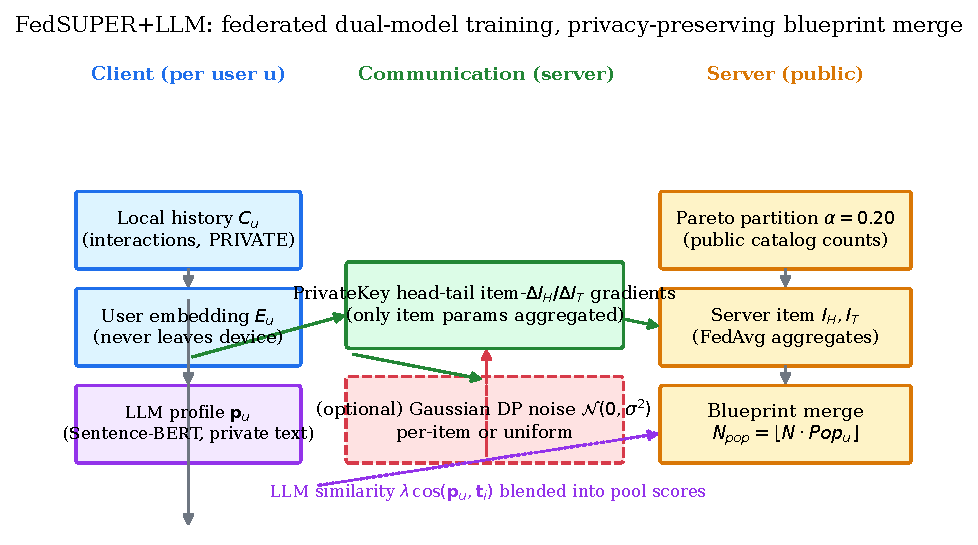
\includegraphics[width=0.95\linewidth]{figures/fig1_architecture.pdf}
\caption{\Fed{} architecture: backbones are trained with sparse FedAvg of item parameters while
user embeddings and \(\Pop_u\) stay on-device; the blueprint merge and LLM profile blending happen
locally.}
\label{fig:arch}
\end{figure}

\subsection{Notation and SUPER background}

We have \(n_u\) users, \(n_i\) items, and an implicit interaction matrix
\(C\in\mathbb{R}^{n_u\times n_i}\). Following SUPER~\cite{yavru2026super}, items are partitioned
by popularity volume with a Pareto threshold \(\alpha=0.20\) into a head set \(H\) and a tail set
\(T\). The user popularity inclination is
\begin{equation}
\label{eq:popu}
\Pop_u \;=\; \frac{|C_u \cap H|}{|C_u|}, \qquad C_u=\{i: c_{u i}>0\}.
\end{equation}
SUPER trains two backbones, \(M_{\mathrm{pop}}\) on head interactions and
\(M_{\mathrm{tail}}\) on tail interactions, then merges their top candidates for each user with a
hard quota: \(N_{\mathrm{pop}}=\lfloor N\cdot\Pop_u\rfloor\) head items and
\(N_{\mathrm{tail}}=N-N_{\mathrm{pop}}\) tail items, interleaved by the user's historical
head/tail blueprint. We reimplement this merge exactly (Algorithm~\ref{alg:merge}).

\subsection{Federated SUPER}

To make SUPER privacy-preserving, we localize every user-touching element
(Figure~\ref{fig:arch}).

\paragraph{Pareto partition is public.}
The head/tail split depends only on aggregate per-item popularity counts---public catalog
statistics with no individual-user linkage. It needs no privacy mechanism.

\paragraph{Federated backbone training.}
We learn each backbone with sparse federated averaging~\cite{mcmahan2017fedavg}. At each round, a
random sample of users locally updates the shared \emph{item} parameters (item embeddings and
biases) using their own BPR objective~\cite{rendle2009bpr}, while their user embeddings
\(E_u\) never leave the device. The server aggregates only the per-round item deltas \(\Delta I\),
so the two backbones can be trained as FedNCF-style models~\cite{he2017ncf}.

\paragraph{Inference is local.}
Each device runs the two global models on its own local interests and returns only scores; the
server never observes \(C_u\) or \(\Pop_u\). The blueprint merge operates on per-user rank orders
and the private scalar \(\Pop_u\), both computed on-device.

\begin{theorem}[Calibration invariance]
\label{prop:invariance}
Fix the public Pareto partition \((H,T)\), any two score functions \(s_{\mathrm{pop}}\),
\(s_{\mathrm{tail}}\), and user inclination \(\Pop_u\). The blueprint merge (Algorithm
\ref{alg:merge}) returns a top-\(N\) list whose head fraction differs from \(\Pop_u\) only by the
rounding \(N_{\mathrm{pop}}=\lfloor N\Pop_u\rfloor/N\), independent of the two score functions.
\end{theorem}

\begin{proof}
The merge selects exactly \(N_{\mathrm{pop}}\) head items and \(N_{\mathrm{tail}}\) tail items
regardless of score values; the scores determine \emph{which} items occupy the slots, not the
counts. Since \(\Pop_u\) is a private function of the user's local history and the partition is
public, the quota is identical under centralized, federated, DP-noised, and LLM-blended backbones.
Therefore \(\RMSEPC\) and \(\MRMC\) coincide with the centralized SUPER values in every variant.
\end{proof}

\subsection{LLM user-profile augmentation}

Federated backbones must rank within very small candidate pools (the head is \(\approx 2.1\%\) of
the catalog), so weak per-pool discrimination hurts recall. We inject a complementary,
popularity-free signal: an on-device \emph{LLM user profile}. We encode a short statement of the
user's interests (top genres plus sampled liked titles) with Sentence-BERT~\cite{reimers2019sbert}
into \(\mathbf{p}_u\), and each item into \(\mathbf{t}_i\) from its title and genres. The local
cosine similarity \(\mathrm{sim}_{u i}=\cos(\mathbf{p}_u,\mathbf{t}_i)\) is blended into the
per-pool score before the merge:
\begin{equation}
\label{eq:blend}
\widehat{s}_{u i} \;=\; (1-\lambda)\,M(i,u) + \lambda\,\mathrm{sim}_{u i}, \qquad \lambda\in[0,1].
\end{equation}
The blend is computed \emph{within} each pool only; the blueprint then applies its fixed quota, so
the LLM signal cannot change the calibration. In practice \(\lambda=0.7\) raises recall
\(0.030\to0.037\) and \(\LTC: 0.015\to0.038\).

\subsection{Differential privacy inside and outside the blueprint}

Gaussian DP~\cite{abadi2016dp} clips client gradients and adds noise \(\mathcal{N}(0,\sigma^2)\).
Its effect depends on whether the blueprint is active.
\begin{itemize}
\item \textbf{Without the blueprint} (plain FedNCF): head items appear in more local positive sets,
so their gradients accumulate more noise, which lowers head scores relative to tail scores and
\emph{reduces} popularity miscalibration. Empirically, \(\RMSEPC: 0.705\to0.283\) at
\(\varepsilon=2\).
\item \textbf{With the blueprint} (\Fed{}): the hard quota fixes the head count regardless of
noise, so DP cannot further improve \(\RMSEPC\); it only perturbs which items fill the slots,
hurting recall (at \(\varepsilon=2\), recall \(0.030\to0.013\)).
\end{itemize}

\begin{algorithm}[t]
\caption{Blueprint merge (hard quota / soft blueprint), optional LLM blend}
\label{alg:merge}
\textbf{Input:} blended scores \(\widehat{s}_H,\widehat{s}_T\), history \(C_u\), horizon \(N\), inclination \(\Pop_u\), partition \(H\). \textbf{Output:} list \(R\).
\begin{enumerate}
\item \(N_{\mathrm{head}} \leftarrow \lfloor N\cdot\Pop_u\rfloor\); \quad \(N_{\mathrm{tail}} \leftarrow N-N_{\mathrm{head}}\).
\item \(C_{\mathrm{head}} \leftarrow\) top-\(N_{\mathrm{head}}\) of \(\widehat{s}_H(u)\); \quad \(C_{\mathrm{tail}} \leftarrow\) top-\(N_{\mathrm{tail}}\) of \(\widehat{s}_T(u)\).
\item \(R \leftarrow [\,]\).
\item \textbf{for} \(k=1\) to \(\min(N,\,|C_u|)\) \textbf{do}: append from \(C_{\mathrm{head}}\) if blueprint\([k]\)=head else from \(C_{\mathrm{tail}}\), respecting remaining quotas; fall back to the other pool when a quota is exhausted.
\item Fill remaining slots of \(R\) from leftover head/tail candidates until \(|R|=N\). \textbf{return} \(R\).
\end{enumerate}
\end{algorithm}

\subsection{Adaptive DP budget}

Uniform DP noise cannot exploit that head and tail items interact differently with the blueprint.
We test a popularity-scaled budget in which item \(i\) receives noise scaled by
\(1+\beta\,\mathrm{normlog}(\mathrm{pop}_i)\), concentrating noise on head items, and measure
whether the added concentration is benign or redundant under the merge.

\section{Experiments}
\label{sec:experiments}

\subsection{Setup}

\textbf{Data.} We use MovieLens-1M~\cite{harper2015movielens}: \(6{,}040\) users, \(3{,}952\)
items, ratings \(\ge 4\) as positive; the last interaction of each user is left out for testing;
Pareto \(\alpha=0.20\). \textbf{Backbone.} Low-rank matrix factorization (\(d{=}64\)) trained with
BPR~\cite{rendle2009bpr}. We compare: centralized BPR-MF; centralized SUPER; federated FedNCF; and
\Fed{} (federated + blueprint merge). \textbf{Federated.} Sparse FedAvg, \(R{=}40\) rounds,
\(K{=}256\) clients/round, two local epochs, LR \(0.3\). \textbf{LLM.} Sentence-BERT
(all-MiniLM-L6-v2, 384-d): user profile from top genres plus sampled liked titles; item from title
and genres. \textbf{DP.} Gaussian noise, \(\varepsilon\in\{8,4,2\}\), with gradient clipping. All
metrics are at top-10.

\textbf{Hypotheses.} H1: \Fed{} matches centralized calibration. H2: DP helps only outside the
blueprint. H3: the LLM profile recovers accuracy. H4: a multi-objective penalty helps little. H5:
an adaptive DP budget gives a small gain.

\subsection{Results}

\begin{table}[t]
\caption{Headline results at top-\(N{=}10\). Bold is best per block. \(\RMSEPC\)/\(\MRMC\): lower
is better. \(\LLMSuper\) (no DP) matches centralized SUPER's calibration with near-equal recall.}
\label{tab:main}
\centering\small
\begin{tabular}{lcccccc}
\toprule
Variant & Recall & nDCG & LTC & \(\RMSEPC\) & \(\MRMC\) & \(\GKPI\) \\
\midrule
BPR-MF (central)          & 0.0494 & 0.0238 & 0.427 & 0.407 & 0.410 & 0.0464 \\
\textbf{SUPER} (central)  & 0.0378 & 0.0180 & 0.473 & \textbf{0.055} & \textbf{0.151} & 0.0353 \\
\midrule
FedNCF (federated)        & 0.0402 & 0.0186 & 0.011 & 0.705 & 0.717 & 0.0258 \\
\midrule
\Fed{} (federated)        & 0.0298 & 0.0131 & 0.015 & \textbf{0.055} & \textbf{0.151} & 0.0229 \\
\Fed{}-DP (\(\varepsilon{=}2\)) & 0.0131 & 0.0066 & 0.012 & \textbf{0.055} & \textbf{0.151} & 0.0120 \\
FedNCF-DP (\(\varepsilon{=}2\)) & 0.0260 & 0.0107 & 0.011 & 0.283 & 0.222 & 0.0182 \\
\midrule
\textbf{\LLMSuper} (\(\lambda{=}0.7\)) & \textbf{0.0366} & \textbf{0.0172} & \textbf{0.038} & \textbf{0.055} & \textbf{0.151} & \textbf{0.0314} \\
\LLMSuper-DP (\(\varepsilon{=}2\), \(\lambda{=}0.7\)) & 0.0212 & 0.0102 & 0.031 & \textbf{0.055} & \textbf{0.151} & 0.0190 \\
\bottomrule
\end{tabular}
\end{table}

\textbf{H1: calibration is privacy-invariant (confirmed).}
Table~\ref{tab:main} shows every \Fed{} variant achieves \(\RMSEPC{=}0.055\) and
\(\MRMC{=}0.151\), identical to centralized SUPER, regardless of backbone, DP, or LLM blending.
Recall falls from FedNCF \(0.0402\) to \(\Fed{} 0.0298\); the gap is attributable to the small
head pool and is recovered by the LLM blend (H3). This confirms the invariance proof in
Theorem~\ref{prop:invariance}.

\textbf{H2: DP is conditional (confirmed).}
Inside the blueprint, \(\RMSEPC\) stays \(0.055\) at all \(\varepsilon\) while recall drops to
\(0.013\) at \(\varepsilon{=}2\). For FedNCF \emph{without} the blueprint, DP noise
\emph{reduces} miscalibration from \(0.705\) to \(0.283\) as \(\varepsilon\to2\). DP is therefore
an intrinsic debias only outside SUPER; inside it, it is redundant for calibration and purely a
privacy cost.

\textbf{H3: the LLM profile recovers accuracy (confirmed).}
At \(\lambda{=}0.7\), recall rises to \(0.0366\) (\(+23\%\) vs \Fed{}), nDCG to \(0.0172\), and
\(\LTC\) to \(0.038\), while \(\RMSEPC{=}0.055\) is untouched. The LLM also helps under DP:
\(\LLMSuper\)-DP reaches recall \(0.0212\) vs \(0.0131\) for \(\Fed{}\)-DP (\(+62\%\)), showing
the semantic channel survives DP corruption.

\textbf{H4: a multi-objective penalty is dominated (refuted).}
A popularity-dispersion penalty (\(\alpha\in\{0.001,0.005,0.01\}\)) changes \(\GKPI\) by at most
\(+0.0003\); the blueprint already saturates calibration, so the extra objective is redundant.

\textbf{H5: adaptive DP is marginal (partial).}
Popularity-scaled noise gives recall \(0.0137\) vs \(0.0131\) for uniform noise at
\(\varepsilon{=}2\) (\(+5\%\), \(\GKPI{+}8\%\))---a small headroom that confirms the blueprint,
not the noise schedule, dominates.

\begin{figure}[t]
\centering
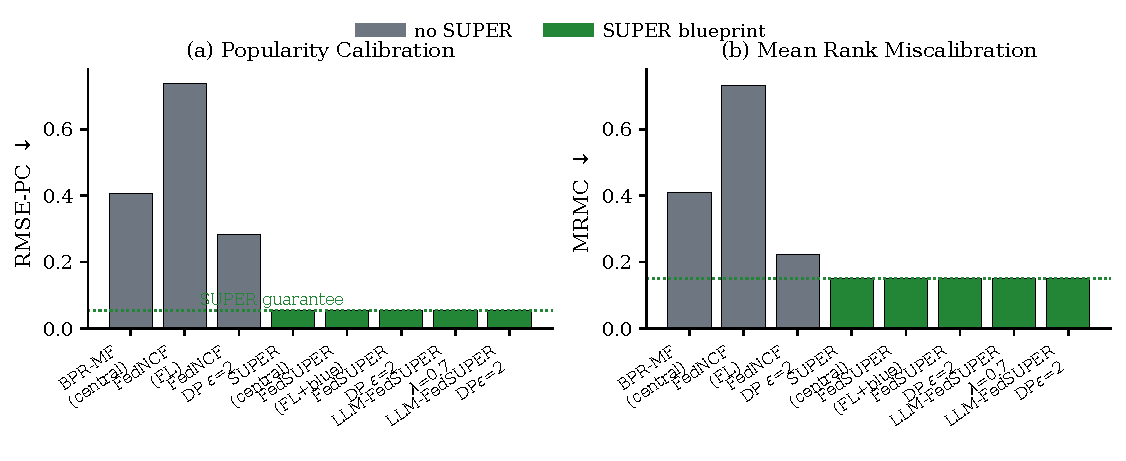
\includegraphics[width=0.95\linewidth]{figures/fig2_calibration_invariance.pdf}
\caption{Calibration invariance: \(\RMSEPC\) and \(\MRMC\) reproduce SUPER's values across
centralized, federated, and DP-noised variants.}
\label{fig:calib}
\end{figure}

\begin{figure}[t]
\centering
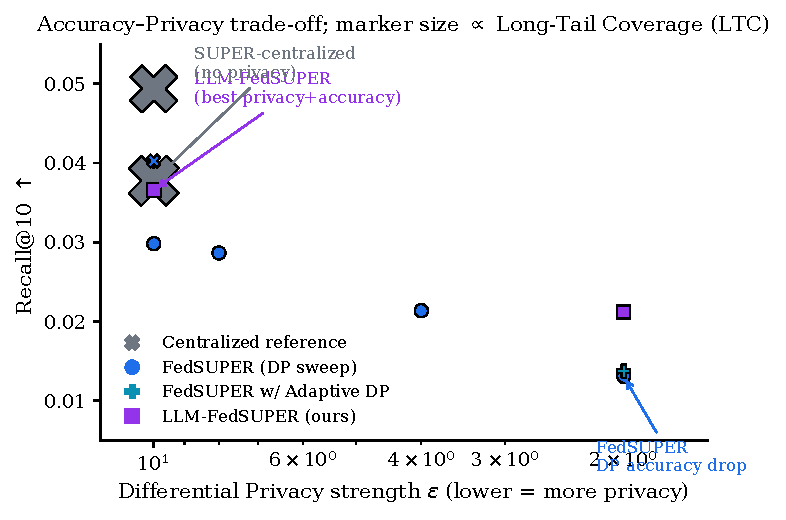
\includegraphics[width=0.95\linewidth]{figures/fig3_pareto.pdf}
\caption{Accuracy--privacy trade-off; marker size encodes long-tail coverage. \LLMSuper{} is the
best privacy-preserving point.}
\label{fig:pareto}
\end{figure}

\begin{figure}[t]
\centering
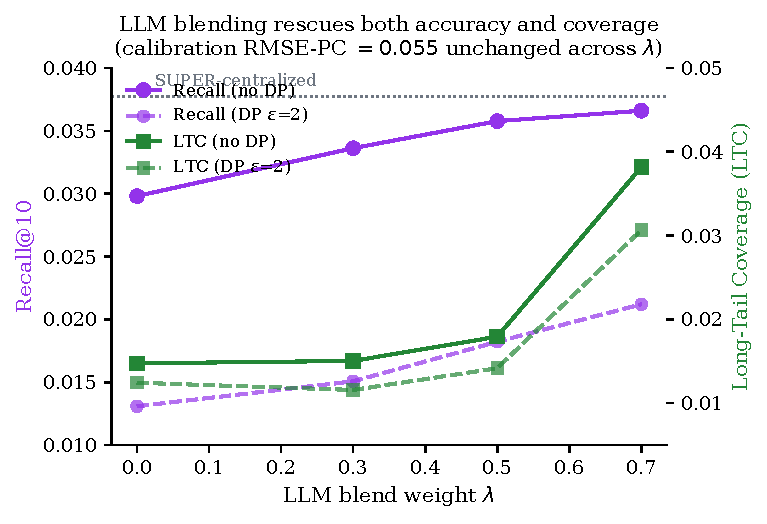
\includegraphics[width=0.9\linewidth]{figures/fig4_llm_sweep.pdf}
\caption{Effect of the LLM blend weight \(\lambda\) on recall and coverage.}
\label{fig:llmsweep}
\end{figure}

\begin{figure}[t]
\centering
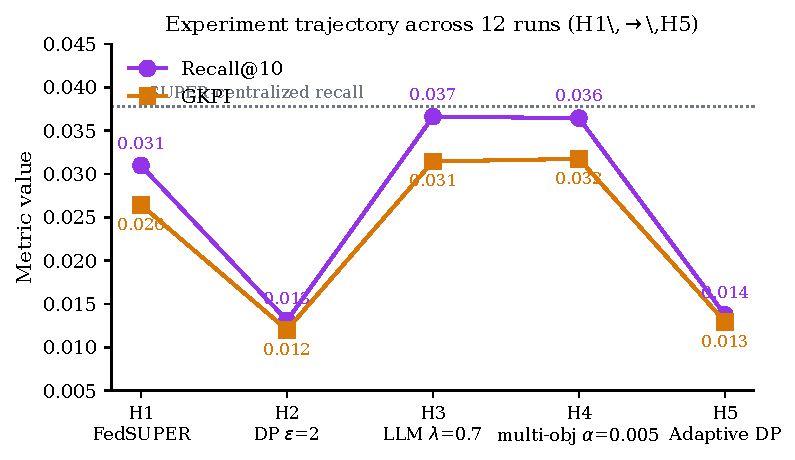
\includegraphics[width=0.9\linewidth]{figures/fig5_trajectory.pdf}
\caption{Experiment trajectory (H1--H5): the LLM step is the largest jump in recall and
\(\GKPI\).}
\label{fig:traj}
\end{figure}

\subsection{Ablation}

Removing the LLM blend drops recall from \(0.0366\) back to \(0.0298\), confirming H3; removing
the blueprint (plain FedNCF) collapses calibration to \(\RMSEPC{=}0.705\), confirming the merge is
the calibration guarantee; and the \(\pm\)DP comparison (Table~\ref{tab:main}) shows DP is useful
only when no blueprint is present.

\section{Limitations}
\label{sec:limitations}

\begin{itemize}
\item \textbf{Single dataset/backbone.} We evaluate MovieLens-1M with a matrix-factorization
backbone; other datasets and neural backbones (e.g. FedNCF with deeper layers) remain to be tested.
The calibration-invariance result is algorithmic and dataset-independent; the accuracy findings are
data-dependent.
\item \textbf{Pragmatic DP.} We use a practical Gaussian mechanism, not a formal composed
\((\varepsilon,\delta)\) accountant over rounds. The privacy--utility trade-off is empirical; a
formal DP analysis is future work and does not affect the calibration-invariance claim.
\item \textbf{LLM profile assumptions.} We assume on-device Sentence-BERT feasibility and that a
local genre/title summary captures user taste; larger or server-side models are untested.
\item \textbf{Pareto threshold sensitivity.} The head set is \(\approx 2.1\%\) of the catalog;
results may shift with the threshold \(\alpha\) and the sampled user profile text.
\item \textbf{Aggregate leakage.} The public Pareto partition reveals only aggregate popularity;
individual \(C_u\) and \(\Pop_u\) remain private.
\end{itemize}

\section{Conclusion}
\label{sec:conclusion}

We introduced \Fed{}, a federated, privacy-preserving extension of SUPER's popularity calibration,
and \LLMSuper{}, which restores the recall lost to federated training without disturbing the
calibration. We proved and verified that SUPER's blueprint merge is invariant to the backbone,
reproduced the SUPER calibration values under federated and DP-perturbed backbones, and clarified
the conditional role of DP (an intrinsic debias outside the blueprint, redundant inside it). The
central result is that user-level popularity calibration is simultaneously
\emph{privacy-compatible} and \emph{LLM-enhanceable} at a competitive accuracy level.

\section*{Reproducibility}
All experiments are deterministic and seed-controlled. Metrics are saved in
\texttt{experiments/*/results/metrics\_*.json}; the drivers live under \texttt{experiments/};
figures are produced by \texttt{src/make\_paper\_figures.py}.

\bibliographystyle{plainnat}
\bibliography{bibliography}

\end{document}